% id: 215-08
% book: 개념원리 중학 3-1 · 23 이차함수의 활용
% section: 중단원 마무리하기 STEP 1 기본 문제
% figure: crop:fig-215-08.png
% answer: ②
% answer_source: 답지
% variant_level: 0 (원본 전사)
% 이 파일은 build.mjs 가 items.json 에서 만든다. 고칠 때는 items.json 을 고친다.
\smash{\raisebox{1.5mm}{\dmkichul{개념원리 중학 3-1 215쪽 08번}}}
\noindent\begin{minipage}[t]{0.58\linewidth}\vspace{0pt}\raggedright 오른쪽 그림과 같은 포물선을 그래프로 하는 이차함수의 식은?\end{minipage}\hfill\begin{minipage}[t]{0.4\linewidth}\vspace{0pt}\centering \setlength{\dmfigw}{75.1pt}\ifdim\dmfigw>\linewidth\setlength{\dmfigw}{\linewidth}\fi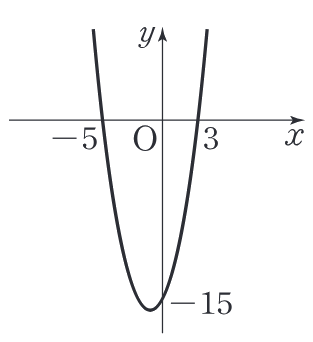
\includegraphics[width=\dmfigw]{figures/fig-215-08.png}\end{minipage}\par
\begin{choicesv}{$y=x^2-2x-15$}{$y=x^2+2x-15$}{$y=x^2-2x+15$}{$y=x^2+2x+15$}{$y=2x^2+4x-15$}\end{choicesv}
